%%
% このファイルは、筑波大学情報学群情報科学類の
% 卒業研究論文本体のサンプルです。
% このファイルを書き換えて、この例と同じような書式の論文本体を
% LaTeXを使って作成することができます。
% 
% PC環境や、LaTeX環境の設定によっては漢字コードや改行コードを
% 変更する必要があります。
%%
\documentclass[a4paper,11pt,dvipdfmx]{jreport}

%%【PostScript, JPEG, PNG等の画像の貼り込み】
%% 利用するパッケージを選んでコメントアウトしてください。
\usepackage{graphicx} % for \includegraphics[width=3cm]{sample.eps}
%\usepackage{epsfig} % for \psfig{file=sample.eps,width=3cm}
%\usepackage{epsf} % for \epsfile{file=sample.eps,scale=0.6}
%\usepackage{epsbox} % for \epsfile{file=sample.eps,scale=0.6}

%% dvipdfm を使う場合(dvi->pdfを直接生成する場合)
%\usepackage[dvipdfm]{color,graphicx}
%% dvipdfm を使ってPDFの「しおり」を付ける場合
%\usepackage[dvipdfm,bookmarks=true,bookmarksnumbered=true,bookmarkstype=toc]{hyperref}
%% 参考:dvipdfm 日本語版
%% http://hamilcar.phys.kyushu-u.ac.jp/~hirata/dvipdfm/

\usepackage[bookmarksnumbered=true]{hyperref}
\usepackage{pxjahyper}

\usepackage{times} % use Times Font instead of Computer Modern

\setcounter{tocdepth}{3}
\setcounter{page}{-1}

\setlength{\oddsidemargin}{0.1in}
\setlength{\evensidemargin}{0.1in} 
\setlength{\topmargin}{0in}
\setlength{\textwidth}{6in} 
%\setlength{\textheight}{10.1in}
\setlength{\parskip}{0em}
\setlength{\topsep}{0em}

%\newcommand{\zu}[1]{{\gt \bf 図\ref{#1}}}

%% タイトル生成用パッケージ(重要)
\usepackage{coins-jp}
\usepackage{jumoline}

%% タイトル
%% 【注意】タイトルの最後に\\ を入れるとエラーになります
\title{\Underline{メソッド本位なオブジェクト指向言語Suzu}}
%% 著者
\author{林 拓人}
%% 指導教員
\advisor{前田敦司}

%% 専攻名 と 年月 (提出年月)
%% 年月は必要に応じて書き替えてください。
\heiseiyear{26}  % 平成の年度
\majorfield{ソフトウェアサイエンス主専攻}
%\majorfield{情報システム主専攻}
%\majorfield{知能情報メディア主専攻}

\makeatletter%% プリアンブルで定義する場合は必須

%% (j)report・(j)book クラスの場合
%% 
\renewenvironment{thebibliography}[1]% 再定義
{\chapter*{\bibname\@mkboth{\bibname}{\bibname}}%
	\addcontentsline{toc}{chapter}{\numberline{}\bibname}% この行追加
	\list{\@biblabel{\@arabic\c@enumiv}}%
	{\settowidth\labelwidth{\@biblabel{#1}}%
		\leftmargin\labelwidth
		\advance\leftmargin\labelsep
		\@openbib@code
		\usecounter{enumiv}%
		\let\p@enumiv\@empty
		\renewcommand\theenumiv{\@arabic\c@enumiv}}%
	\sloppy
	\clubpenalty4000
	\@clubpenalty\clubpenalty
	\widowpenalty4000%
	\sfcode`\.\@m}
{\def\@noitemerr
	{\@latex@warning{Empty `thebibliography' environment}}%
	\endlist}

\makeatother%% プリアンブルで定義する場合は必須


\begin{document}
\maketitle
\thispagestyle{empty}
\newpage

\thispagestyle{empty}
\vspace*{20pt plus 1fil}
\parindent=1zw
\noindent
%%
%% 論文の概要(Abstract)
%%
\begin{center}
{\Large \bf 要  旨}
\vspace{2cm}
\end{center}
[400字程度]

%%%%%
\par
\vspace{0pt plus 1fil}
\newpage

\pagenumbering{roman} % I, II, III, IV 
\tableofcontents
\listoffigures
%\listoftables

\pagebreak \setcounter{page}{1}
\pagenumbering{arabic} % 1,2,3


\chapter{序論}



オブジェクトシステムとは,\textbf{オブジェクト指向プログラミング}\cite{Stroustrup:1988:OP:624569.624721}
を支援するプログラミング言語の機構である.
本研究は従来のオブジェクトシステムのモデル化を通じて考案した,新しいモデルに基づくオブジェクトシステムを
提案する.
従来とは異なるモデルによって,オブジェクトシステムにまつわる既存の概念に対し新たな見方を提示することが
目的である.

[ここで論文の構成について述べる]


\chapter{従来のオブジェクトシステム}
\label{chapter:conventional}

本研究は従来のオブジェクトシステムのうち,\textbf{クラスにメソッドを定義するもの}と
\textbf{総称関数にメソッドを定義するもの}に注目した.
本章ではこの2種類のメソッド定義の方式をモデル化する.

\section{クラスにメソッドを定義するモデル}

Smalltalk,C++,Java,Rubyなどの言語に組み込まれているオブジェクトシステムでは,\textbf{クラス}に
所属する形でメソッドを定義する.
これは図\ref{figure:class-model}のようにモデル化することができる.メソッド定義のコード例にはRubyを
用いている.

\begin{figure}[htbp]
	\centering
	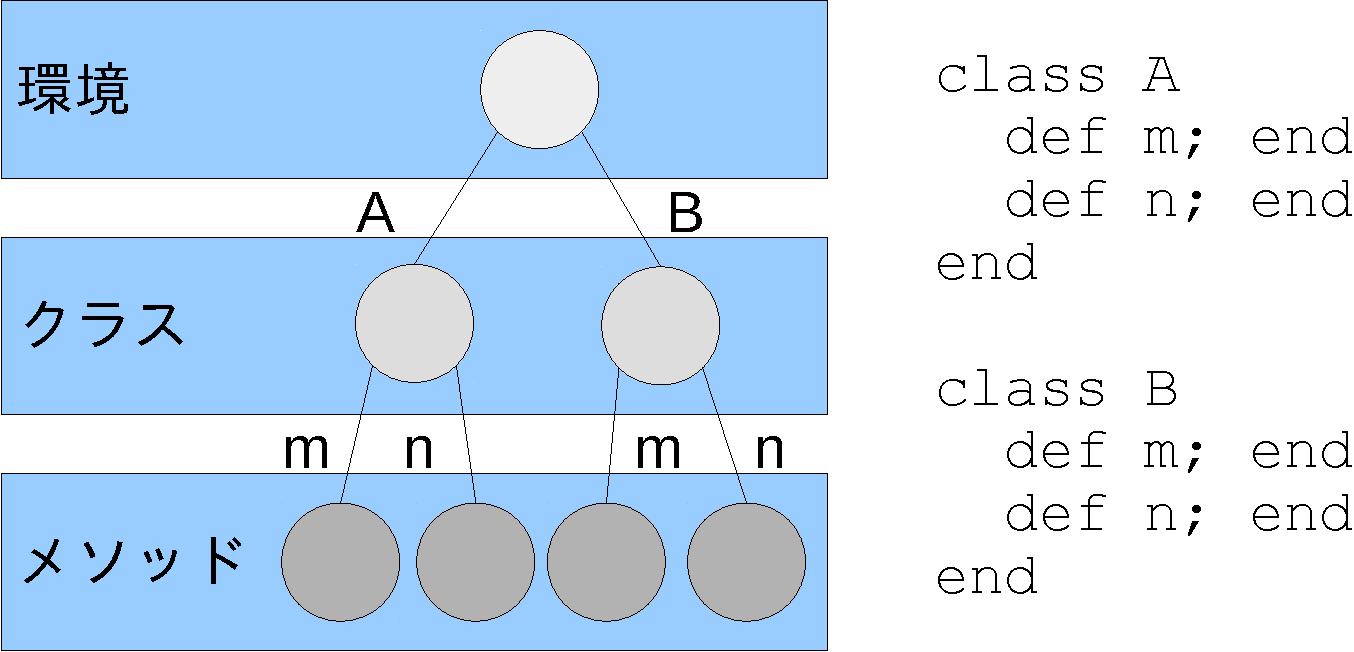
\includegraphics[width=9cm]{fig/trees_class-crop.pdf}
	\caption{クラスにメソッドを定義するモデル(例:Ruby)}
	\label{figure:class-model}
\end{figure}

\textbf{環境}は名前と値の対応関係の集合である.
ここではクラス名とクラスを対応付ける\textbf{クラス環境}を指す.
このモデルでは環境にクラスを定義し,クラスにメソッドを定義する.
図\ref{figure:class-model}では環境を根とする木構造によってモデルを表現している.
環境からクラスへと伸びる枝はクラス名によってラベル付けされ,クラスからメソッドへと伸びる枝はメソッド名によって
ラベル付けされる.
このモデルにおいてメソッドはまずクラス名によって分類され,次にメソッド名によって分類されるという2段階の分類が
行われているといえる.

\section{総称関数にメソッドを定義するモデル}

Common Lisp,Dylanなどの言語に組み込まれているオブジェクトシステムでは,\textbf{総称関数}に
所属する形でメソッドを定義する.
これは図\ref{figure:gf-model}のようにモデル化することができる.メソッド定義のコード例にはCommon Lispを
用いている.
\verb|defmethod|はメソッドを同名の総称関数に追加する.もし総称関数が定義されていなければ
新しく生成する.
総称関数は複数のメソッドを束ねる関数で,与えられた引数のクラスに応じて適切なメソッドを選択し呼び出す.

\begin{figure}[htbp]
	\centering
	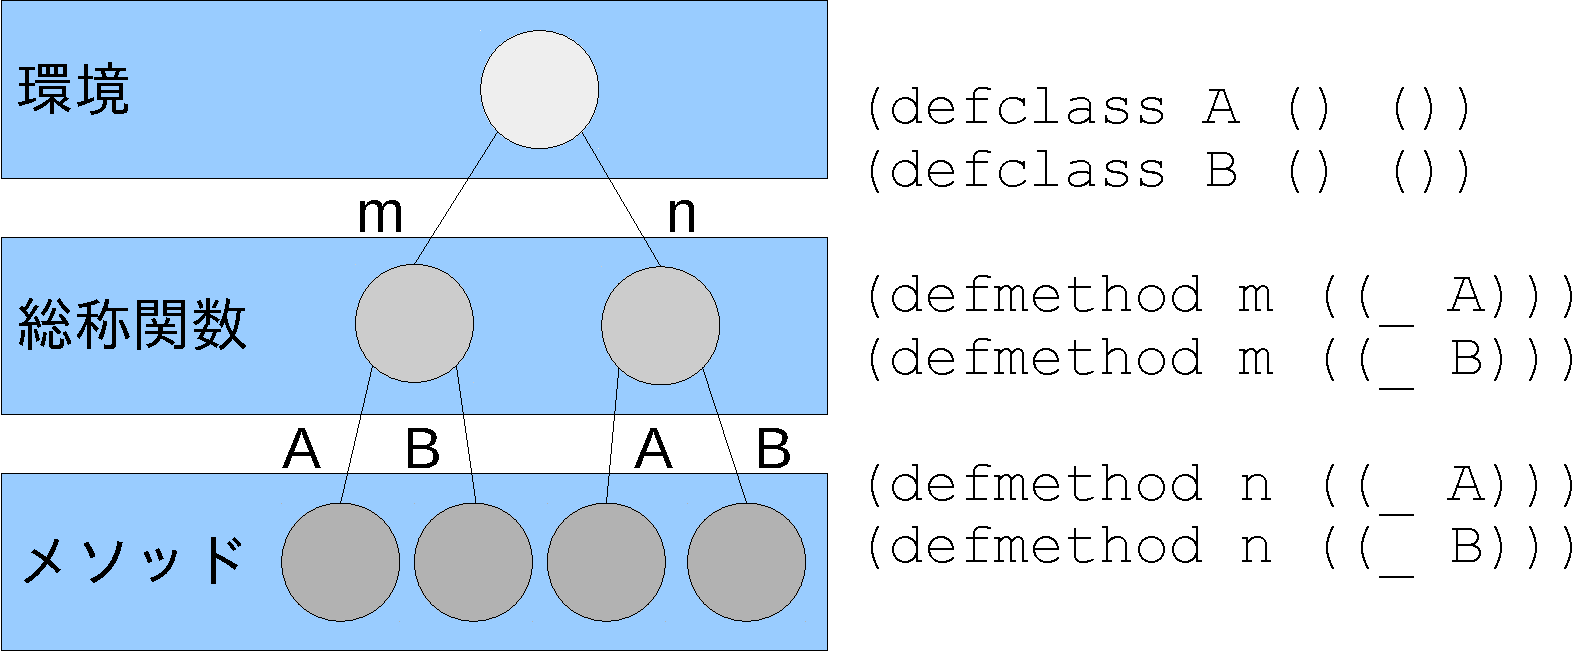
\includegraphics[width=10cm]{fig/trees_gf-crop.pdf}
	\caption{総称関数にメソッドを定義するモデル(例:Common Lisp)}
	\label{figure:gf-model}
\end{figure}

ここでの環境は関数名と関数を対応付ける\textbf{関数環境}を指す.
このモデルでは環境に総称関数を定義し,総称関数にメソッドを定義する.
図\ref{figure:gf-model}では図\ref{figure:class-model}と同様,環境を根とする木構造によって
モデルを表現している.
環境から総称関数へと伸びる枝はメソッド名(=総称関数名)によってラベル付けされ,総称関数からメソッドへと
伸びる枝はクラス名によってラベル付けされる.
このモデルにおいてメソッドはまずメソッド名によって分類され,次にクラス名によって分類されるという,
図\ref{figure:class-model}と同じ2段階の分類が行われているといえる.

なおここではモデルを単純化するため,総称関数が1つの引数のクラスに応じてメソッドを選択する
\textbf{単一ディスパッチ}に限定して考え,総称関数からメソッドへと伸びる枝を1つのクラス名のみでラベル付け
している.
Common Lispは複数の引数のクラスに応じてメソッドを選択する\textbf{多重ディスパッチ}に対応しているが,
これについては考慮していない.

[多重ディスパッチについて書いた章へのrefを載せるかも]

\section{分析}

図\ref{figure:class-model}と図\ref{figure:gf-model}を比較すると,
どちらもメソッドをクラス名とメソッド名という2つの要素によって,順序の違う2段階の分類を行っている.
そして1段目の分類を行うために,概念上クラスまたは総称関数というメソッドを格納する\textbf{コンテナ}の
存在を仮定している.
このコンテナはあくまで概念上のものだが,しばしば実際に処理系の実装にも現れる.


\chapter{提案するオブジェクトシステム}

第\ref{chapter:conventional}章でモデル化した2種類のオブジェクトシステムは,
メソッドを格納するコンテナとしてのクラスまたは総称関数の存在を仮定し,メソッドをクラス名とメソッド名によって
2段階に分けて分類していた.
本章ではこの代替となりうるメソッド定義モデル,およびそれに基づく新しいオブジェクトシステムを提案する.

\section{環境にメソッドを直接定義するモデル}

図\ref{figure:class-model}および図\ref{figure:gf-model}の代替となりうるメソッドの分類方法として,
図\ref{figure:containerlsss-model}のような木構造が考えられる.
これをメソッド定義モデルとしてとらえると,\textbf{環境にメソッドを直接定義するモデル}であるといえる.

\begin{figure}[htbp]
	\centering
	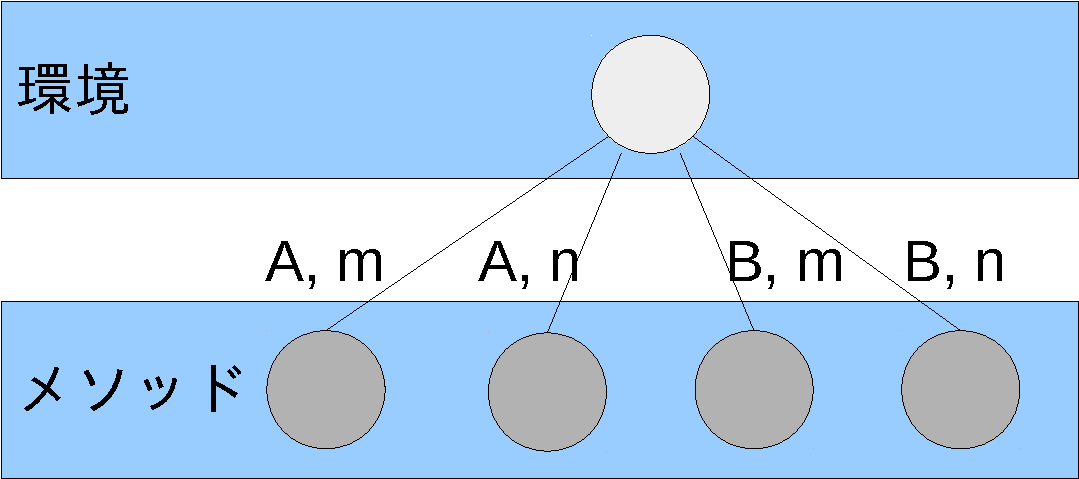
\includegraphics[width=7cm]{fig/trees_containerless-crop.pdf}
	\caption{環境にメソッドを直接定義するモデル}
	\label{figure:containerlsss-model}
\end{figure}

環境からメソッドへと伸びる枝は\textbf{クラス名とメソッド名の組}によってラベル付けされる.
第\ref{chapter:conventional}章で述べた2つのモデルがメソッドをクラス名とメソッド名によって
2段階に分けて分類していたのに対し,このモデルではクラス名とメソッド名の組による1段階のみの分類を行う.
このためメソッドのコンテナとしてのクラスや総称関数の存在を仮定する必要はない.
本稿ではこの特徴にちなんで,このモデルに基づくオブジェクトシステムを
\textbf{Containerlsssなオブジェクトシステム}と呼ぶ.

\section{Containerlessなオブジェクトシステム}

Containerlessなオブジェクトシステムとはコンテナとしてのクラスや総称関数を用いず
環境にメソッドを直接定義するオブジェクトシステムの総称である.
ここでいう環境とは,クラス名とメソッド名の組をメソッドに対応付けるものである.

Containerlessなオブジェクトシステムという単語が規定するのはこのメソッド定義モデルのみであり,
その他の要素によって様々なバリエーションが考えられる.
第\ref{chapter:suzu}章ではContainerlessなオブジェクトシステムの実装例として
独自言語Suzuを紹介し,第\ref{chapter:discussion}章で


\chapter{実装:プログラミング言語Suzu}
\label{chapter:suzu}

\chapter{考察}
\label{chapter:discussion}

クラスは

\chapter{結論}

従来のオブジェクトシステムのうちクラスにメソッドを定義するものと総称関数にメソッドを定義するものの
モデル化を通じ,環境にメソッドを直接定義する新しいメソッド定義モデルContainerlessを考案した.
Containerlessなメソッド定義モデルに基づくオブジェクトシステムの例として独自に設計したプログラミング言語
Suzuに実装した.


\chapter*{謝辞}
\addcontentsline{toc}{chapter}{\numberline{}謝辞}

本研究を行うにあたり多大なるご指導とご助言を下さった筑波大学システム情報系前田敦司准教授に
深く感謝いたします.
また第56回プログラミング・シンポジウムにて本研究に対するコメントを下さった方々に
感謝いたします.
最後に貴重なご意見を下さった筑波大学インタラクティブ・アーキテクチャ研究室の皆様とOBの水島宏太さんに
感謝いたします.

\newpage

%\addcontentsline{toc}{chapter}{\numberline{}参考文献}
\renewcommand{\bibname}{参考文献}

%% 参考文献に jbibtex を使う場合
\bibliographystyle{junsrt}
\bibliography{thesis}
%% [compile] jbibtex sample; platex sample; platex sample;

%% 参考文献を直接ファイルに含めて書く場合
%\begin{thebibliography}{1}
%\bibitem{RakRak}
%野寺隆志.
%\newblock 楽々 \LaTeX.
%\newblock 共立出版, 1990.
%
%\bibitem{JiyuuJizai}
%磯崎秀樹.
%\newblock \LaTeX 自由自在.
%\newblock サイエンス社, July 1992.
%
%\bibitem{bryant-ieeetc86}
%Randal~E. Bryant.
%\newblock Graph-based algorithms for {B}oolean function manipulation.
%\newblock {\em IEEE Transactions on Computers}, Vol. C-35, No.~8, pp. 677--691,
%  August 1986.
%\end{thebibliography}

\end{document}
